\clearpage{}
\section{Define software architecture, software units, architectural views.
Describe the following architectural styles: pipes-and-filter,
client-server, peer-to-peer, publish-subscribe, repositories, layering.}

\subsection{Define}

\subsubsection{Software architecture/design}

Software architecture refers to the high level structures of a software
system. We now focus on the HOW to implement the customer's requirement
(not on the WHAT). The system's architecture is structural, systemic and
hard to change.

\paragraph{Sources of design}

\begin{figure}[!ht]
    \centering
    \begin{tikzpicture}[node distance=3cm, on grid, auto]
    \node[draw, ellipse] (design) {Design};
    \node[above = 2cm of design] (simsys) {Similar systems};
    \node[above right = 1.5cm and 3.5cm of design] (refmod) {Reference models};
    \node[below right = 1.5cm and 3.5cm of design] (archstyle) {Architectural styles};
    \node[below right = 3cm and 1cm of design] (despat) {Design patterns};
    \node[below left = 3cm and 2.5cm of design] (desconv) {Design conventions};
    \node[below left = 0.5cm and 4cm of design] (despr) {Design principles};
    \node[above left = 1.5cm and 3cm of design] (exp) {Experience};

    \path[->, line width=2pt] (simsys) edge node {} (design);
    \path[->, line width=2pt] (refmod) edge node {} (design);
    \path[->, line width=2pt] (archstyle) edge node {} (design);
    \path[->, line width=2pt] (despat) edge node {} (design);
    \path[->, line width=2pt] (desconv) edge node {} (design);
    \path[->, line width=2pt] (despr) edge node {} (design);
    \path[->, line width=2pt] (exp) edge node {} (design);
\end{tikzpicture}

    \caption{Sources of design}
\end{figure}

\paragraph{The design process}

\begin{figure}[!ht]
    \centering
    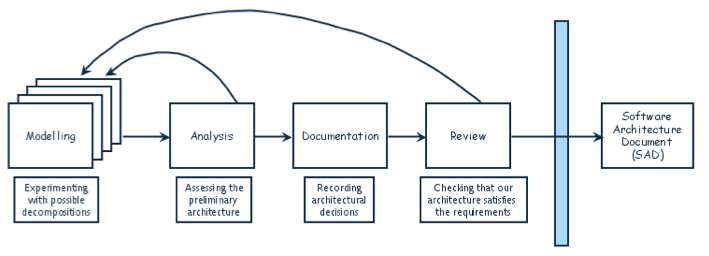
\includegraphics[width=\linewidth]{design_process.png}
    \caption{The design process}
\end{figure}


\subsubsection{Software units}

Architecture design decomposes the system into software units (depending on
aspects considered):

\begin{itemize}
    \item Components
    \item Classes
    \item Subsystems
    \item Packages
    \item Runtime processes
    \item Libraries
    \item Modules
    \item Procedures
\end{itemize}


A design is modular when each activity of the system is performed by exactly one
software unit (the inputs and outputs of each software unit are well-defined).

A software unit is well-defined when its externally visible behaviour is
precisely specified.

\subsubsection{Architectural views}

In addition to decompose the system in software units, the system could be
analysed with different architectural views. Common types of architectural views:

\begin{description}
    \item[Decomposition view (traditional view)] portrays the system as
    programmable units (typically a hierarchy of models)
    \item[Dependencies view] shows dependencies among software units (useful in
    project planning)
    \item[Generalization view] shows software units that are generalizations or
    specializations of one another (useful when designing abstract or extendible
    software units)
    \item[Execution view] shows the runtime structure of a system in terms of
    its components and connectors (the traditional box-and-arrow diagram)
    \item[Implementation view] maps software units to source files (helps
    programmers find implementations)
    \item[Deployment view] maps runtime entities to computer resources (helps
    the architect analyse the quality attributes)
    \item[Work-assignment view] decomposes the design into work tasks (helps
    project managers to plan and allocate project resources and to track each
    team's progress)
\end{description}


\subsection{Architectural styles}

\subsubsection{Pipes-and-filter}

\begin{figure}[!ht]
    \centering
    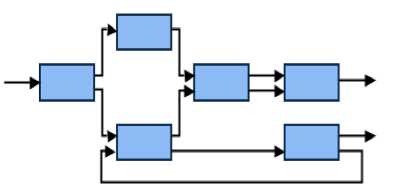
\includegraphics[width=0.3\linewidth]{pipes_and_filter.png}
    \caption{Pipes and filter}
\end{figure}

In a pipe-and-filter style, system functionality is achieved by passing input
data through a sequence of data-transforming components, called filters, to
produce output data. Pipes are connectors that simply transmit data from one
filter to the next without modifying the data.

\begin{itemize}
    \proitem{} Reason by functional composition
    \proitem{} Filters can be reused easily
    \proitem{} Easy evolution: add, replace, remove filters
    \proitem{} Allow concurrent execution of filters
    \proitem{} Compositional throughput analysis
    \consitem{} Overhead of parsing inputs, producing outputs
    \consitem{} Batch processing, not good for interactive
\end{itemize}

\subsubsection{Client-server}

\begin{figure}[!ht]
    \centering
    \footnotesize
    \begin{tikzpicture}[node distance = 2cm, on grid, auto]
    \node[draw, rectangle] (appserv) {Application server};
    \node[draw, rectangle, below of = appserv] (db) {Database server};
    \node[draw, ellipse, above of = appserv] (wb2) {\begin{tabular}{c}Web\\browser\end{tabular}};
    \node[draw, ellipse, left = 3cm of wb2] (wb1) {\begin{tabular}{c}Web\\browser\end{tabular}};
    \node[draw, ellipse, right = 3.5cm of wb2] (desk) {\begin{tabular}{c}Desktop\\application\end{tabular}};
    \node[right = 7.5cm of wb2]  (client) {Client presentation};
    \node[right = 7.1cm of appserv] (business) {Business logic};
    \node[right = 7.5cm of db] {Information system};

    \path[<->, line width=2pt] (db) edge node  {} (appserv);
    \path[<->, line width=2pt] (wb1) edge node  {} (appserv);
    \path[<->, line width=2pt] (wb2) edge node  {} (appserv);
    \path[<->, line width=2pt] (desk) edge node  {} (appserv);
\end{tikzpicture}

    \caption{Client-server architecture}
\end{figure}

Servers offer services and clients access them using a request/reply protocol.
Note that clients know servers but servers don't know clients.

\begin{itemize}
    \proitem{} Can distribute servers among processors $\rightarrow$ improve
    performance
    \proitem{} Servers can be layered (multitier)
    \proitem{} Supports reuse of servers across applications
\end{itemize}

\subsubsection{Peer-to-peer (P2P)}
\begin{figure}[!ht]
    \centering
    \begin{scriptsize}
        \section{Peer-to-Peer}

\subsection{Overview P2P systems}
P2P computing is distributed computing  with the following desirable properties:
\begin{itemize}
	\item Resource sharing
	\item Dual client/server role
	\item Decentralization/autonomy
	\item Scalability
	\item Robustness/self-organization
\end{itemize}

\subsection{Distributed Hash Table}

DHT are third generation of P2P:

\begin{tabular}{m{10cm}m{6cm}}
\begin{itemize}
    \item a dynamic distribution of a hash table onto a set of cooperating nodes.
        (different node contains different parts of the table).
    \item Each node has a routing table that points to some other nodes.
    \item Lookup operation is done by node to make a key resolution
\end{itemize}
&
    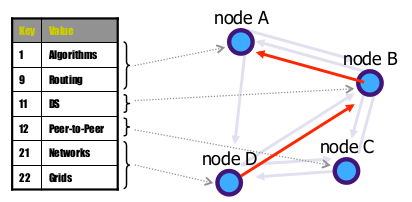
\includegraphics[width=6cm]{img/DHT.png}

     \textcolor{red}{Node D: lookup(9)}\\
    \\
\end{tabular}

\begin{lstlisting}[caption=Interface DHT]
put(key,value).
get(key)
\end{lstlisting}

\subsubsection{Chord}

\begin{tabular}{m{10cm}m{3cm}m{3cm}}
\begin{itemize}
    \item \textbf{Routing table size} $= M$ s.t $N = 2^M$
    \item Every node $n$ know successor $(n + 2^{i-1})$ for $i = 1..M$
    \item $log_2(N)$ maximum hops between two node
\end{itemize}
& 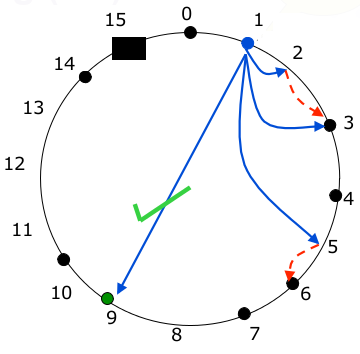
\includegraphics[width=3cm]{img/chord.png}
& 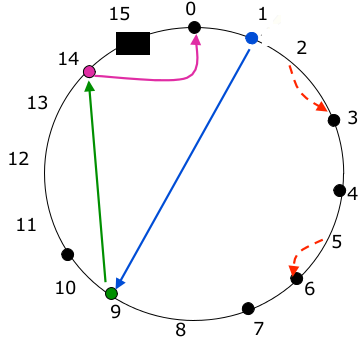
\includegraphics[width=3cm]{img/chord1.png}\\
& \multicolumn{2}{c}{$\Rightarrow$ 1 get(15)}
\end{tabular}

\subsubsection{Generally}

\begin{itemize}
    \item We have $N$ node
    \item[$\to$] Trade-off between lookup length and routing table size

   \begin{eqnarray*}
            H &= log_k(N)\\
            R &=(k-1) H \\
            N &= (\frac{R}{H} + 1)^H\\
        \end{eqnarray*}
\end{itemize}

Chord is a special case where $k=2$.

\subsubsection{DKS}

\begin{itemize}
    \item Tunability: \begin{tabular}{l}
            Routing table size vs lookup length\\
            fault-tolerance degree
        \end{tabular}
    \item Local atomic join and leave (strong guarantees)
    \item Correction-on-use : no unnecessary bandwith consumption
\end{itemize}

\subsubsection{Design DKS(n, k, f)}
\begin{tabular}{m{10cm}m{3cm}m{3cm}}
\begin{itemize}
    \item An \textbf{identifier space} of size $N=k^L$
    \item A hash function
    \item An item ($key, value$) is stored at \textbf{successor} of
        H(key)
    \item \textbf{Bidirectional} linked list of nodes
    \item Resolving key : $\bigoh(N) hops$
\end{itemize}
& 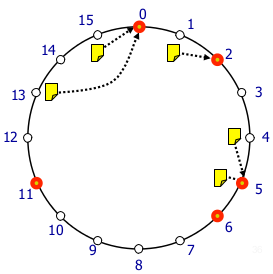
\includegraphics[width=3cm]{img/dks1.png}
& 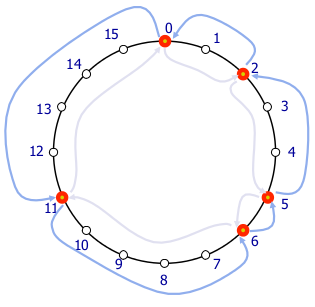
\includegraphics[width=3cm]{img/dks2.png} \\
\end{tabular}


\paragraph{Principle}

\begin{enumerate}
    \item \textbf{Distributed K-ary search}:
        \begin{itemize}
            \item resolution key: $log_k(N)$ hops
            \item At each node, a $RT$ of $\log_k(N)$ level
            \item Each level of $RT$ has $k$ intervals
            \item For level $l$ ant interval $i$: $RT(l)(i) = $ adress of the fist node
                that follow the start of the interval $i$
        \end{itemize}

        \paragraph{Interval routing}
        \begin{enumerate}
            \item If key between my predecessor and me: done
            \item Otherwise systematic forwarding level by level
        \end{enumerate}

        \paragraph{Example with $k=4$, $N=16$}:

        \begin{tabular}{m{6cm}m{6cm}m{4cm}}

            \begin{center}\textcolor{purple}{Level 1} \end{center}
            \begin{eqnarray*}
                I_0 &= [1, 5[ &: RT(1)(0) = 1\\
                I_1 &= [5, 9[ &: RT(1)(1) = 6\\
                I_2 &= [9, 13[ &: RT(1)(2) = 10\\
                I_3 &= [13, 1[ &: RT(1)(3) = 15\\
            \end{eqnarray*}
            &
            \begin{center}\textcolor{green}{Level 2} \end{center}
            \begin{eqnarray*}
                I_0 &= [1, 2[ &: RT(2)(0) = 1\\
                I_1 &= [2, 3[ &: RT(2)(1) = 2\\
                I_2 &= [3, 4[ &: RT(2)(2) = 3\\
                I_3 &= [4, 5[ &: RT(2)(3) = 6\\
            \end{eqnarray*}

            & 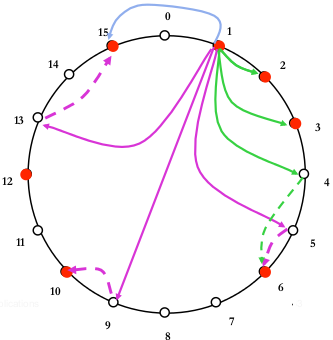
\includegraphics[width=4cm]{img/design1.png}
        \end{tabular}


    \item \textbf{Local atomic action for guarantees}:

        Use local atomic operation for \textbf{join, leave} to ensure
        that any key-value pair previously inserted is found despite concurrent
        joins/leaves.

        \begin{enumerate}
            \item Atomically insterted by it's current successor on the virtual space
            \item New node receive approximate routing information from it's current successor
            \item[$\to$] Concurrent join on the same segment are serialized (because of local
                atomic action)
        \end{enumerate}

        \begin{tabular}{m{10cm}m{4cm}}

            \begin{itemize}
                \item Node 14 join
                \item Pointer for node 1 on level=1 interval=3 become invalid
                \item[$\to$] corrected by correction-on-use
            \end{itemize}

            & 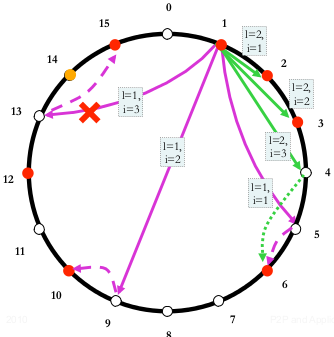
\includegraphics[width=4cm]{img/design2.png}
        \end{tabular}

    \item \textbf{Correction-on-use}:

        \begin{tabular}{m{10cm}m{4cm}}
            Add i (interval) and l (level) with the message
            $\Rightarrow$ $n'$ can comppute $x_i^l(n)$

            \begin{itemize}
                \item[a)] lookup(Key:13, level:1, Interval:3)
                \item[b)] badPointer(Key:13, Candidate:14)
                \item[c)] lookup(Key:13, level:1, Interval:3)
            \end{itemize}

            & 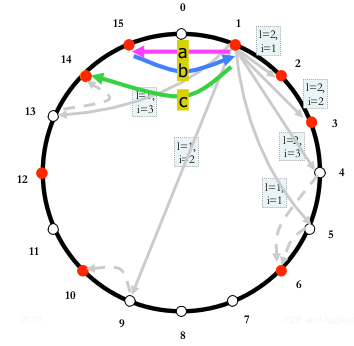
\includegraphics[width=4cm]{img/design3.png}
        \end{tabular}
\end{enumerate}


\subsection{Broadcast in DHTs}

\begin{itemize}
    \item \textbf{DHT as distributed k-ary search}: construct a spanning tree
        derived from the decision tree of the distributed k-ary search after removal
        of the virtual hops

        \paragraph{Invariant}:
        \begin{itemize}
            \item Any node sends to distinct routing entries
            \item Any sender informs receiver about a \textbf{forwarding limit}
            \item[$\to$] Construct disjoint interval and node receives a message once
        \end{itemize}

        \begin{figure}[!ht]
            \centering
            \begin{tabular}{m{4cm}m{4cm}m{4cm}}
                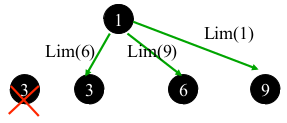
\includegraphics[width=4cm]{img/DHT1.png}
                & 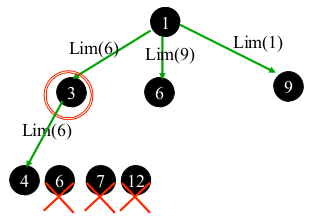
\includegraphics[width=4cm]{img/DHT2.png}
                & 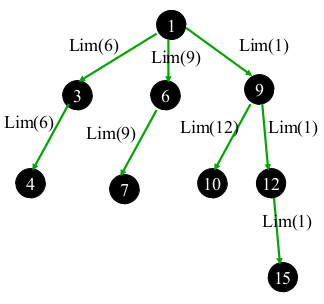
\includegraphics[width=4cm]{img/DHT3.png}\\
            \end{tabular}
            \caption{DHD spanning tree}
        \end{figure}
        \FloatBarrier{}

    \item[Alternative]

    \item \textbf{Gnutella-like flooding in DHT}:
        \begin{itemize}
            \item[Pro] know diameter $\to$ correct TTL $\to$ High guarantees
            \item[Con] High traffic with redundant messages
        \end{itemize}

    \item \textbf{Traversing the ring in Chord or Pastry}:
        \begin{itemize}
            \item[Pro] No redundant message
            \item[Con] Sequential execution time
            \item[Con] Highly sensitive to failure
        \end{itemize}
\end{itemize}


\subsection{Application infrastructure in DHT}
%TODO

    \end{scriptsize}
    \caption{Peer-to-peer architecture}
\end{figure}

All components are peers (equals), they execute concurrently and act as both
clients and servers (i.e.\ specify both provided and requested services).
\newline
In other words, any component can call any component.

\begin{itemize}
    \proitem{} Scale up well
    \proitem{} Increased system capabilities (replication)
    \proitem{} Highly tolerant of failures (replication)
\end{itemize}

\subsubsection{Publish-subscribe}

\begin{figure}[!ht]
    \centering
    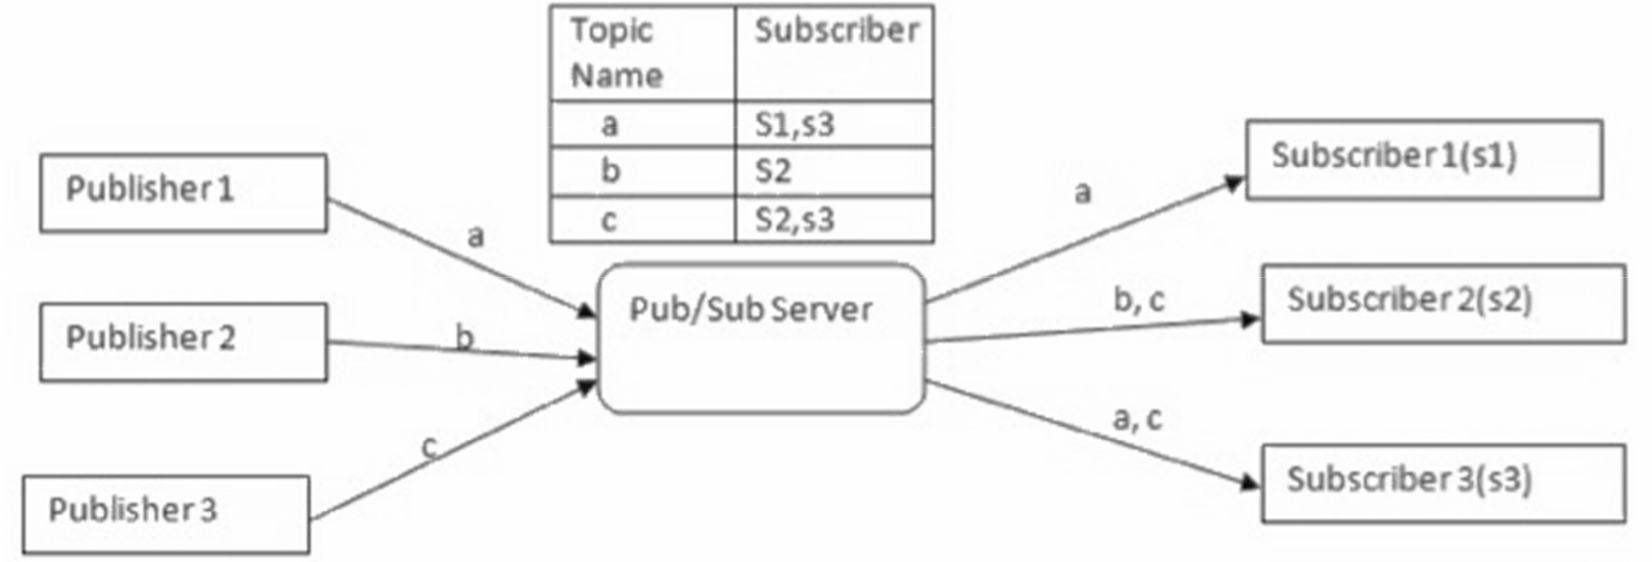
\includegraphics[width=0.6\linewidth]{publish_suscribe.png}
    \caption{Publish-subscribe architecture}
\end{figure}

Subscribers subscribe to events from a server (bus) by registering a callback
(implicit invocation). Publishers publish (broadcast) events to the server
(bus). Registered subscribers receive the events (the server calls the
callback).\newline
Note that publishers and subscribers don't know each other (all know the server
and the events).

\begin{itemize}
    \proitem{} Easy evolution, customization, reuse
    \consitem{} Need shared repository for shared persistent data
    \consitem{} Difficult to test
\end{itemize}

\subsubsection{Repositories}

\begin{figure}[!ht]
    \centering
    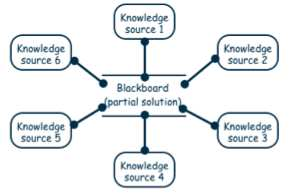
\includegraphics[width=0.5\linewidth]{repositories.png}
    \caption{Repositories architecture}
\end{figure}

A repository style of architecture consists of two types of components: a
central data store and associated data-accessing components. 
Shared data are
stockpiled in the data store, and the data accessors are computational units
that store, retrieve, and update the information. \newline

In a traditional database, components are active (clients) and data store is
reactive. In the blackboard type of repository, blackboard (data store) is
active and knowledge sources (components) are reactive.

\begin{itemize}
    \proitem{} Centralized management of data
    \proitem{} Improve performance (distribute)
    \consitem{} More complex, consistency, security (distribute)
\end{itemize}

\subsubsection{Layering}

\begin{figure}[!ht]
    \centering
    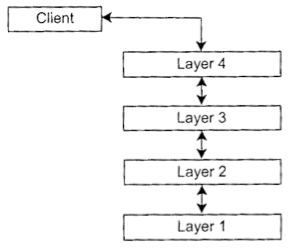
\includegraphics[width=0.3\linewidth]{layering.png}
    \caption{Layering architecture}
\end{figure}

Layered systems organize the system’s software units into layers, each of which
provides services to the layer above it and acts as a client to the layer below.
We can thus say that each layer raises the level of abstraction.

\begin{itemize}
    \proitem{} Relatively easy to add or modify a layer
    \proitem{} Porting on different platforms
    \consitem{} Not applicable to all systems
    \consitem{} System performance may suffer extra coordination among layers
\end{itemize}
